\documentclass[11pt]{article}
\usepackage[margin=0.72in]{geometry}
\usepackage{xcolor}
\usepackage{tikz}
\usetikzlibrary{positioning}
\usepackage{graphicx}
\usepackage{enumitem}
\usepackage{hyperref}
\usepackage{titlesec}
\usepackage{tcolorbox}
\definecolor{ink}{HTML}{121212}
\definecolor{paper}{HTML}{F5F3EE}
\definecolor{action}{HTML}{0E7C66}
\definecolor{warn}{HTML}{B15D16}
\hypersetup{colorlinks=true, linkcolor=action, urlcolor=action}
\pagecolor{paper}
\color{ink}
\titleformat{\section}{\Large\bfseries\color{action}}{}{0em}{}
\setlist[itemize]{leftmargin=1.4em, itemsep=0.25em}

\begin{document}

\begin{center}
{\Huge \textbf{Project Panopticon}}\\[0.35em]
{\Large Zero-Escalation Support through Adversarial Multi-Agent Orchestration}\\[0.75em]
{\small Hackathon Gold-Tier Submission}
\end{center}

\begin{tcolorbox}[colback=white,colframe=action,arc=2mm,boxrule=0.8pt]
\textbf{Core idea:} A customer escalation should not trigger a chatbot. It should trigger a private war room. Panopticon runs Support, Customer Care, and Sales agents in parallel, then lets ContextGuard attack their drafts before a single customer-facing word is released.
\end{tcolorbox}

\section{Why It Matters}
Enterprise escalations combine technical failure, churn risk, and commercial opportunity. Traditional bots flatten those into one generic answer. Panopticon separates the concerns, lets specialized agents reason independently, and uses an adversarial adjudicator to prevent hallucinations, policy violations, and tone mistakes.

\section{Architecture}
\begin{center}
\resizebox{\textwidth}{!}{%
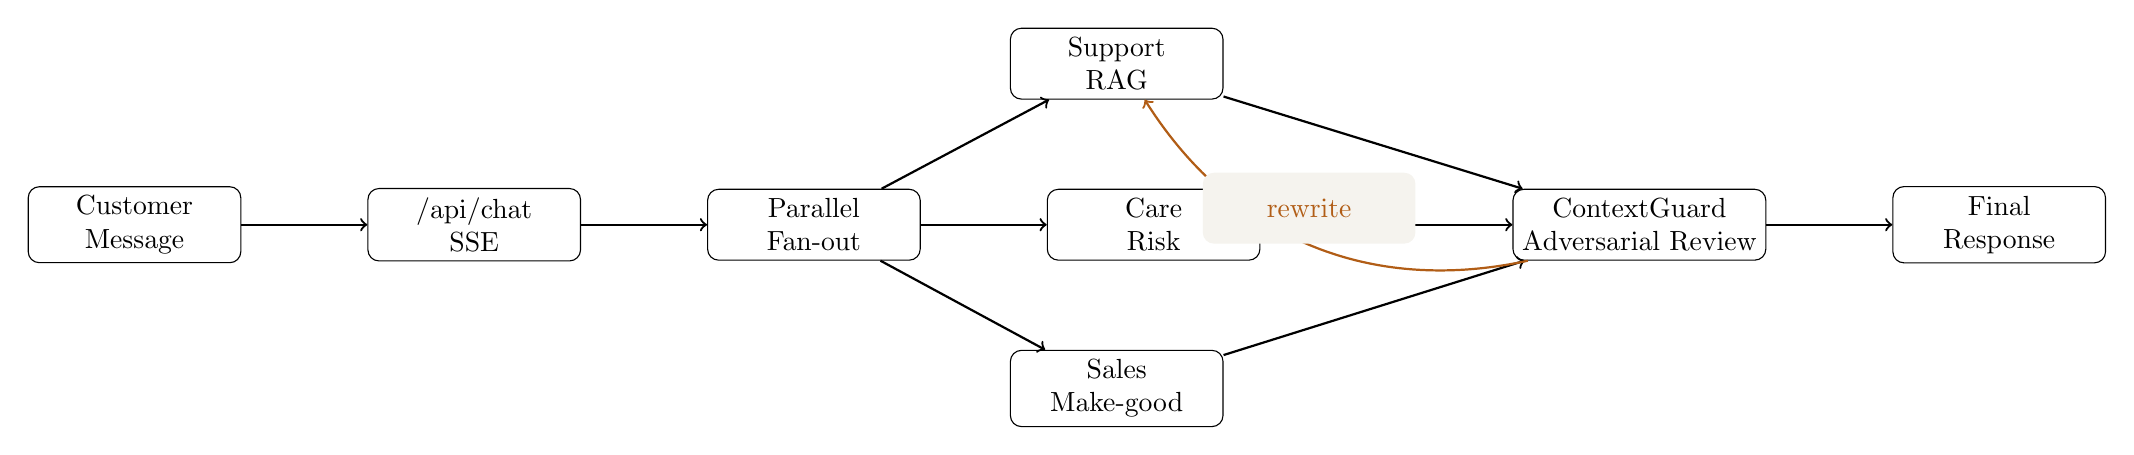
\begin{tikzpicture}[node distance=1.6cm, every node/.style={draw, rounded corners, align=center, fill=white, minimum width=2.7cm, minimum height=0.9cm}]
\node (u) {Customer\\Message};
\node[right=of u] (api) {/api/chat\\SSE};
\node[right=of api] (fan) {Parallel\\Fan-out};
\node[above right=of fan] (support) {Support\\RAG};
\node[right=of fan] (care) {Care\\Risk};
\node[below right=of fan] (sales) {Sales\\Make-good};
\node[right=3.2cm of care] (guard) {ContextGuard\\Adversarial Review};
\node[right=of guard] (final) {Final\\Response};
\draw[->, thick] (u) -- (api);
\draw[->, thick] (api) -- (fan);
\draw[->, thick] (fan) -- (support);
\draw[->, thick] (fan) -- (care);
\draw[->, thick] (fan) -- (sales);
\draw[->, thick] (support) -- (guard);
\draw[->, thick] (care) -- (guard);
\draw[->, thick] (sales) -- (guard);
\draw[->, thick] (guard) -- (final);
\draw[->, thick, bend left=35, color=warn] (guard) to node[above, draw=none, fill=paper] {rewrite} (support);
\end{tikzpicture}
}
\end{center}

\section{Implemented Features}
\begin{itemize}
\item Split-screen Next.js interface with customer chat on the left and a streaming Live War Room terminal on the right.
\item Local vector database built from a synthetic enterprise knowledge base.
\item Parallel Support, Care, and Sales agents with strict TypeScript schemas.
\item ContextGuard adversarial review with forced rewrite when a deprecated API key appears.
\item Churn scoring and automatic 20\% SLA credit guardrail.
\item Contextual Enterprise make-good offer when the technical problem maps to active-active failover.
\item Sales suppression for Enterprise customers and unsupported/trick-question flows.
\item Server-Sent Events streaming for logs, drafts, guardrail decisions, and final output.
\item OpenAPI documentation at \texttt{/api/openapi} plus local architecture and prompt docs.
\item Remotion composition for programmatic product video generation.
\item Automated tests for retrieval, churn scoring, rewrite behavior, and demo cases.
\end{itemize}

\section{Evaluation Alignment}
\begin{tcolorbox}[colback=white,colframe=ink,arc=2mm,boxrule=0.6pt]
\textbf{Innovation:} Panopticon is an adversarial operating loop, not a single chatbot prompt.\\
\textbf{Technical Architecture:} DAG orchestration, SSE streaming, local RAG, caching, strict schemas, and provider integration points.\\
\textbf{Support:} Grounded fix generation with self-correction.\\
\textbf{Customer Care:} Predictive churn scoring and bounded SLA credit.\\
\textbf{Sales:} Crisis-aware make-good upsell only when useful and appropriate.\\
\textbf{Documentation:} README, architecture diagram, prompts, OpenAPI, screenshots, demo script, and this submission package.
\end{tcolorbox}

\section{Demo Moment}
The strongest demo prompt is: \textit{``Your API crashed again and my payment gateway is down. I'm taking my business elsewhere!''} The Live War Room shows Support drafting a risky deprecated key instruction, ContextGuard blocking it, Support rewriting the fix, and the customer receiving a safe answer with \texttt{gateway\_failover=true}, \texttt{Idempotency-Key}, and \texttt{/v3/status/incidents}.

\end{document}
